\documentclass[9pt,twoside,lineno]{pnas-new}
% Use the lineno option to display guide line numbers if required.

\templatetype{pnassupportinginfo}

\title{Water resource utilization regimes at a basin scale: transition framework and development traps}
\author{Shuang Song, Shuai Wang, Bojie Fu, Xutong Wu (complete author list)}
\correspondingauthor{Shuai Wang.\\E-mail: shuaiwang@bnu.edu.cn}

\begin{document}

%% Comment out or remove this line before generating final copy for submission; this will also remove the warning re: "Consecutive odd pages found".
% \instructionspage

\maketitle

%% Adds the main heading for the SI text. Comment out this line if you do not have any supporting information text.
\SItext test


% \subsection*{Brief description of Supplementary Information contents: }
% Type or paste text here. This should be additional explanatory text such as an extended technical description of results, full details of mathematical models, etc.   

% \section*{Supplementary Information Methods}
\section*{Methods S1. Definition of study area}
% 黄河经历了水资源开发利用和制度改革
The study area is the Yellow River Basin (YRB), 
which has experienced the most intense water exploitation 
and the most dramatic reform of management regimes.

\subsection*{Introduction of Yellow River Basin}
\subsection*{Subarea of Yellow River Basin}
\subsection*{General situation of water use in the YRB}

\section*{Methods S2. Detailed information on dataset and processing}
Add a materials' subsection if you need to.

\section*{Methods S3. Water Utilization Regime Index}
Add a methods subsection if you need to.


%%% Each figure should be on its own page
\begin{figure}
\centering
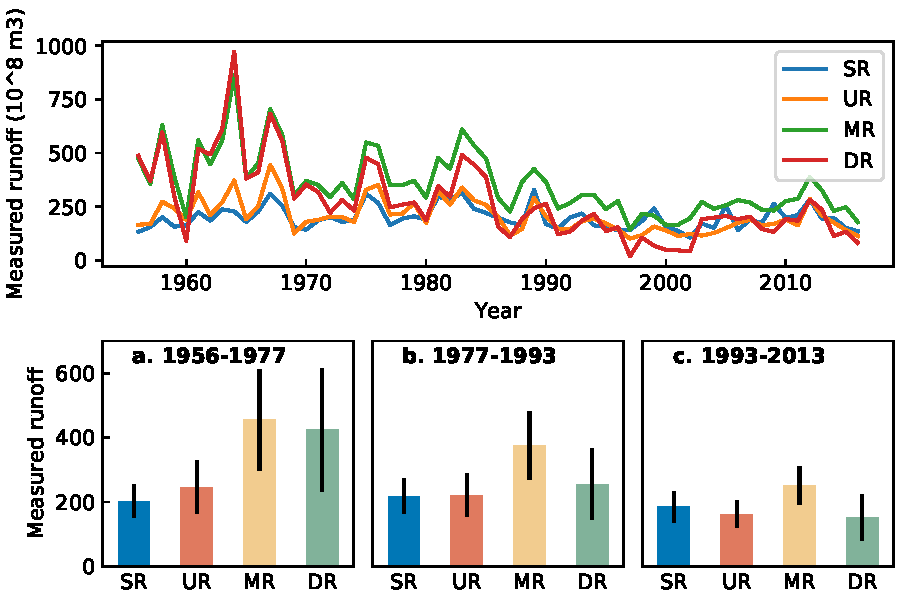
\includegraphics[width=\textwidth]{../../figures/supplementary_information/sf_measured_runoff.pdf}
\caption{Natural measured runoff of Yellow River within different periods.}
\end{figure}

\begin{figure}
\centering
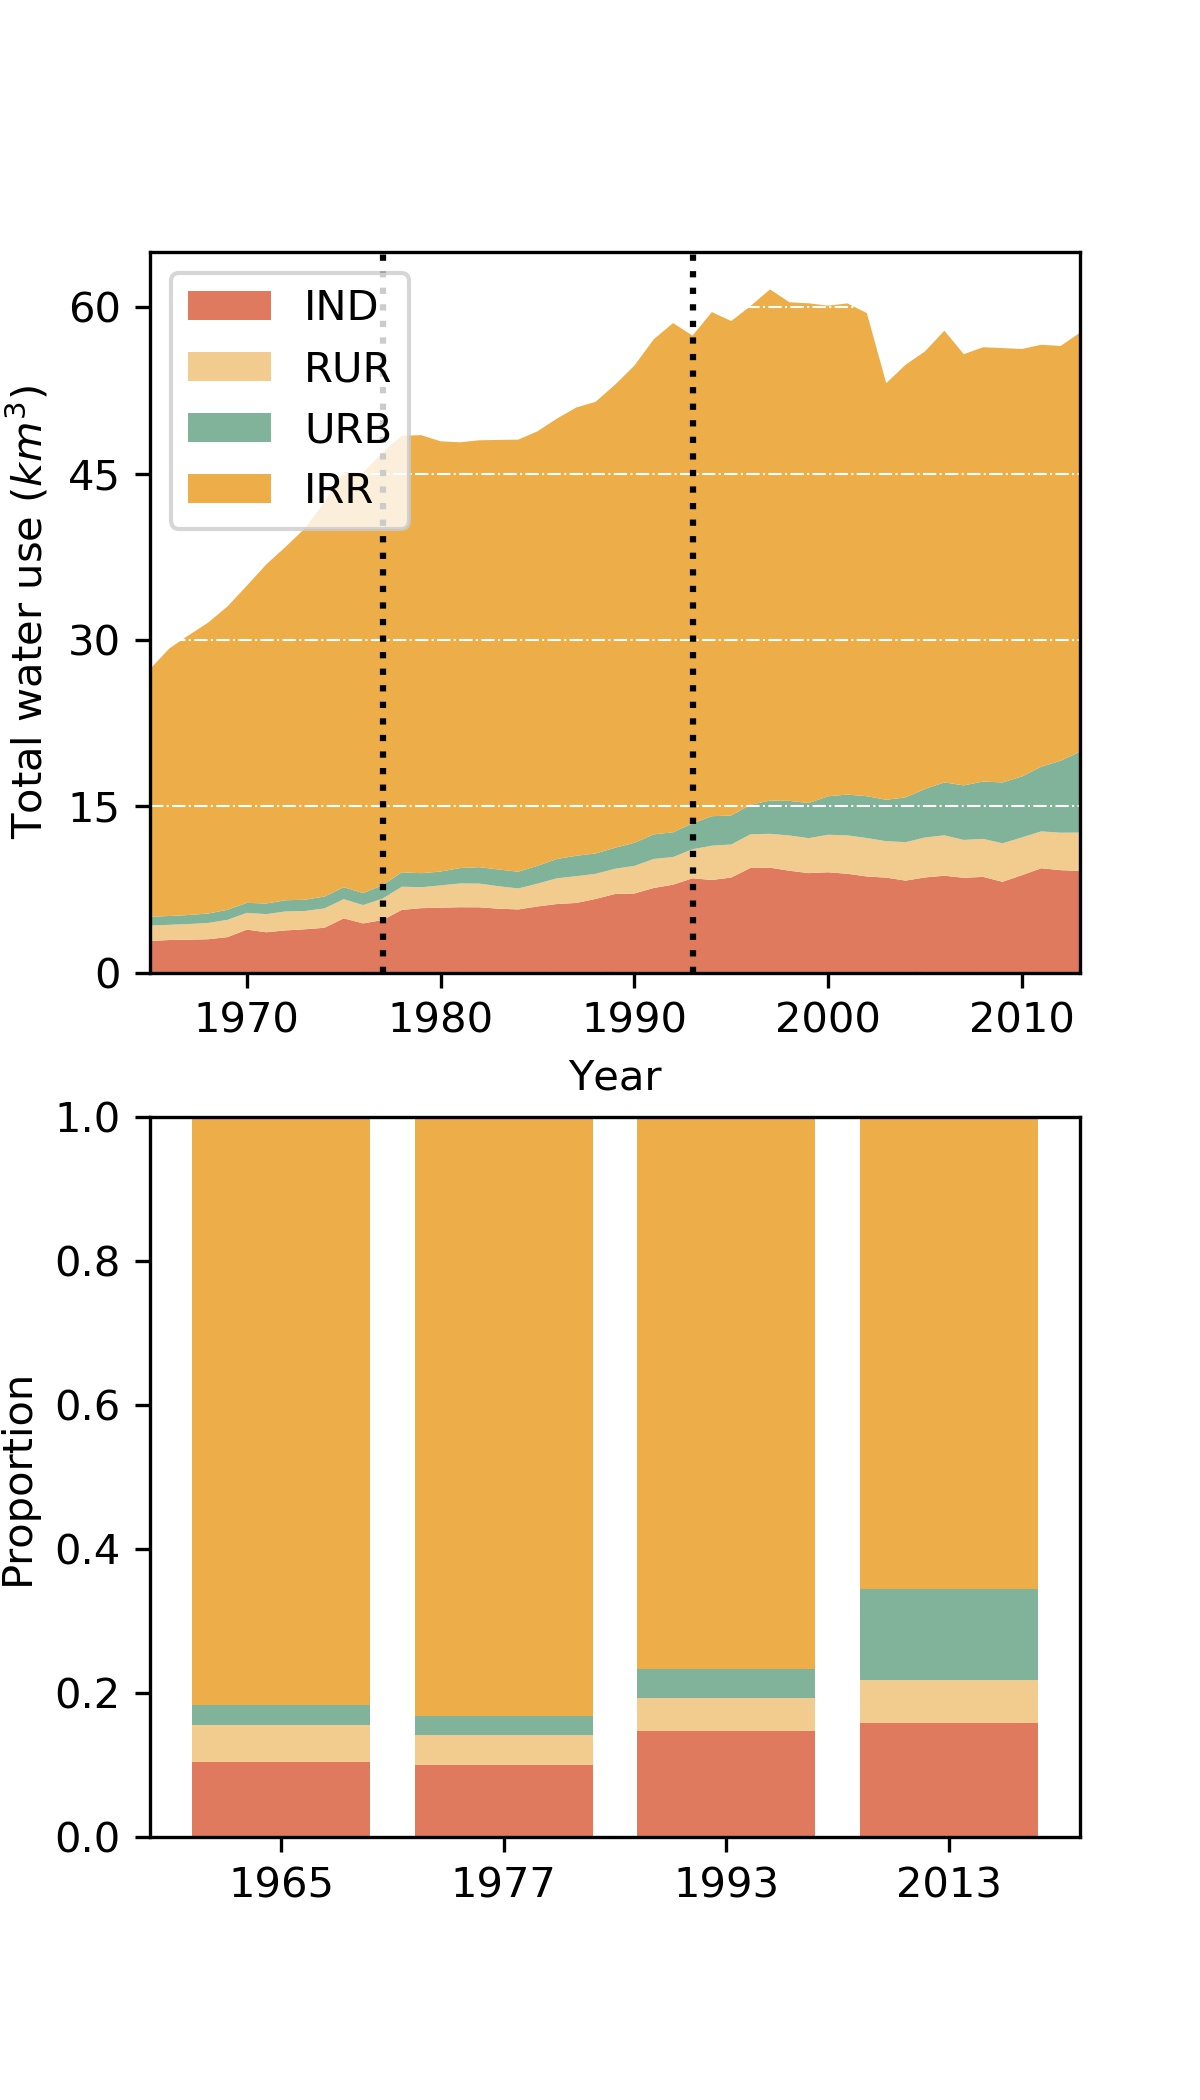
\includegraphics[width=\textwidth]{../../figures/supplementary_information/sf_wu_sections_stackplot.jpg}
\caption{Second figure}
\end{figure}

\begin{table}\centering
\caption{This is a table}

% 表格
\begin{tabular}{lrrr}
Species & CBS & CV & G3 \\
\midrule
1. Acetaldehyde & 0.0 & 0.0 & 0.0 \\
2. Vinyl alcohol & 9.1 & 9.6 & 13.5 \\
3. Hydroxyethylidene & 50.8 & 51.2 & 54.0\\
\bottomrule
\end{tabular}
\end{table}




%%% Add this line AFTER all your figures and tables
\FloatBarrier

\dataset{dataset_one.txt}{Type or paste legend here.}

\dataset{dataset_two.txt}{Type or paste legend here. Adding longer text to show what happens, to decide on alignment and/or indentations for multi-line or paragraph captions.}

\bibliography{pnas-sample}

\end{document}